\chapter{Implementation}
\begin{comment}
    - Github? forskjellige repo?
    - External data / sources used for map, etc.
\end{comment}

\textcolor{orange}{NOE TEKST}

\section{Technologies}

This section provides a structured overview of the technologies employed in the project, along with a rationale for their selection.

\subsection{TypeScript}

% https://www.typescriptlang.org/docs/handbook/intro.html
TypeScript is a statically typed superset of JavaScript that adds optional type annotations and other features to improve code quality and maintainability. While JavaScript is popular for both frontend and backend development, it lacks built-in mechanisms to express relationships between components as applications grow. This often leads to runtime errors, many of which are related to incorrect or unexpected types. TypeScript addresses these issues by providing a static type system that checks for such errors during development, before the code is executed. By catching mistakes early and offering better tooling and autocomplete support, TypeScript makes large-scale JavaScript applications easier to develop, refactor, and maintain \cite{typescript_handbook}. 

For these reasons TypeScript was chosen to implement the website. All libraries written in JavaScript like OpenLayers and React could be used, but with the added type-safety of TypeScript.

\subsection{React}

React is a JavaScript library designed for rendering user interfaces (UI), where everything on the screen, from buttons to images, can be broken down into small, reusable components. These components are the building blocks of React, allowing you to create, customize, and conditionally display content across your application \cite{react_component}. As your application scales, it becomes increasingly important to manage the state effectively and ensure that data flows smoothly between components. Poorly organized or redundant state can lead to bugs, so React encourages a structured approach to state management. React makes it easy to share states between components \cite{react_state}. 

Using React when developing the website made it much easier and time-efficient which was important for this project. 

\subsection{OpenLayers}

OpenLayers is a JavaScript library used for displaying and interacting with geographic data on web maps. It provides an extensive and well documented set of tools for working with vector and raster data, supporting various formats such as \Gls{geojson}, \Gls{wms}, and \Gls{wfs}. OpenLayers allows developers to create highly customizable and interactive maps with features like layer control, coordinate projections, and dynamic styling \cite{openlayers}.

The website uses OpenLayers to render image layers for \gls{superficial deposit}s, soil moisture, and \gls{frost} depth, and display vector features like forestry roads.  

\subsection{Web Map Service and Web Feature Service}

% NEVNE SPESIFIKKE FUNKSJONER (GetFeatureInfo / GetMap) ?
Web Map Service (\Gls{wms}) and Web Feature Service (\Gls{wfs}) are both standards developed by the Open Geospatial Consortium to facilitate the distribution of geographic information over the web. A WMS generates dynamic maps from spatially referenced data, rendering them as digital images in formats such as PNG, GIF, and JPEG. WMS allows users to request maps that specify geographic regions, desired coordinate systems, and map dimensions. There are also queryable WMS services that enable users to retrieve metadata about the map and its features at specific coordinates. Additionally, \Gls{wms} supports the creation of composite maps by layering different map images, with transparency in formats like PNG and GIF, allowing the underlying maps to be visible \cite{ogc2006wms}.

In contrast, a WFS enables the retrieval of raw geographic data, such as vector features, from a web server. Unlike \Gls{wms}, which provides static map images, \Gls{wfs} allows users to request feature-level data in formats like \Gls{geojson}, enabling more interactive and detailed analyses. WFS supports spatial queries and provides access to vector-based geographic features, such as points, lines, and polygons, which can be used for advanced geospatial analysis and integration into other systems. While WMS is ideal for visualizing spatial data, WFS is better suited for manipulating raw geospatial data \cite{ogc2005wfs}.

In the implementation of this product, both WMS and WFS are used to visualize and interact with geospatial data. For example, the superficial deposits and frost depth layers utilize WMS to display these datasets as map images on the web interface. On the other hand, the forestry road layer is implemented using WFS, providing access to vector-based geographic features as lines. This allows further processing, such as determining \gls{trafficability} or road conditions. Additionally, when querying a single coordinate, the Superficial Deposits layer uses the query operation to retrieve information about the specific location, ensuring that users can obtain feature data at precise geographic points.

\section{Website}

This section contains an overview of the implementation of the website.

\begin{comment}
    - Typescript & React (vite/template, code structure?)
        - Template: npm create vite@latest myapp -- --template react-ts
    - OpenLayers
    - GUI-elements
    - Map layers and legends
    - Forestry road vector layer
    - Datepicker / temporal aspect of map layers
\end{comment}

\subsection{Wireframe} % Vet ikke om dette burde være et annet sted?

A wireframe of the website was made to agree on the layout of the website and the required features. \hyperref[fig:wireframe_website_sidebars_closed]{Figure \ref*{fig:wireframe_website_sidebars_closed}} shows the basic layout of the website including the map and the date picker. In \hyperref[fig:wireframe_website_sidebars_opened]{Figure \ref*{fig:wireframe_website_sidebars_opened}} it shows the sidebars for both enabling map layers and their legends. Additionally it shows a layer being enabled and querying that feature for additional information.

\begin{figure}[h]
    \centering
    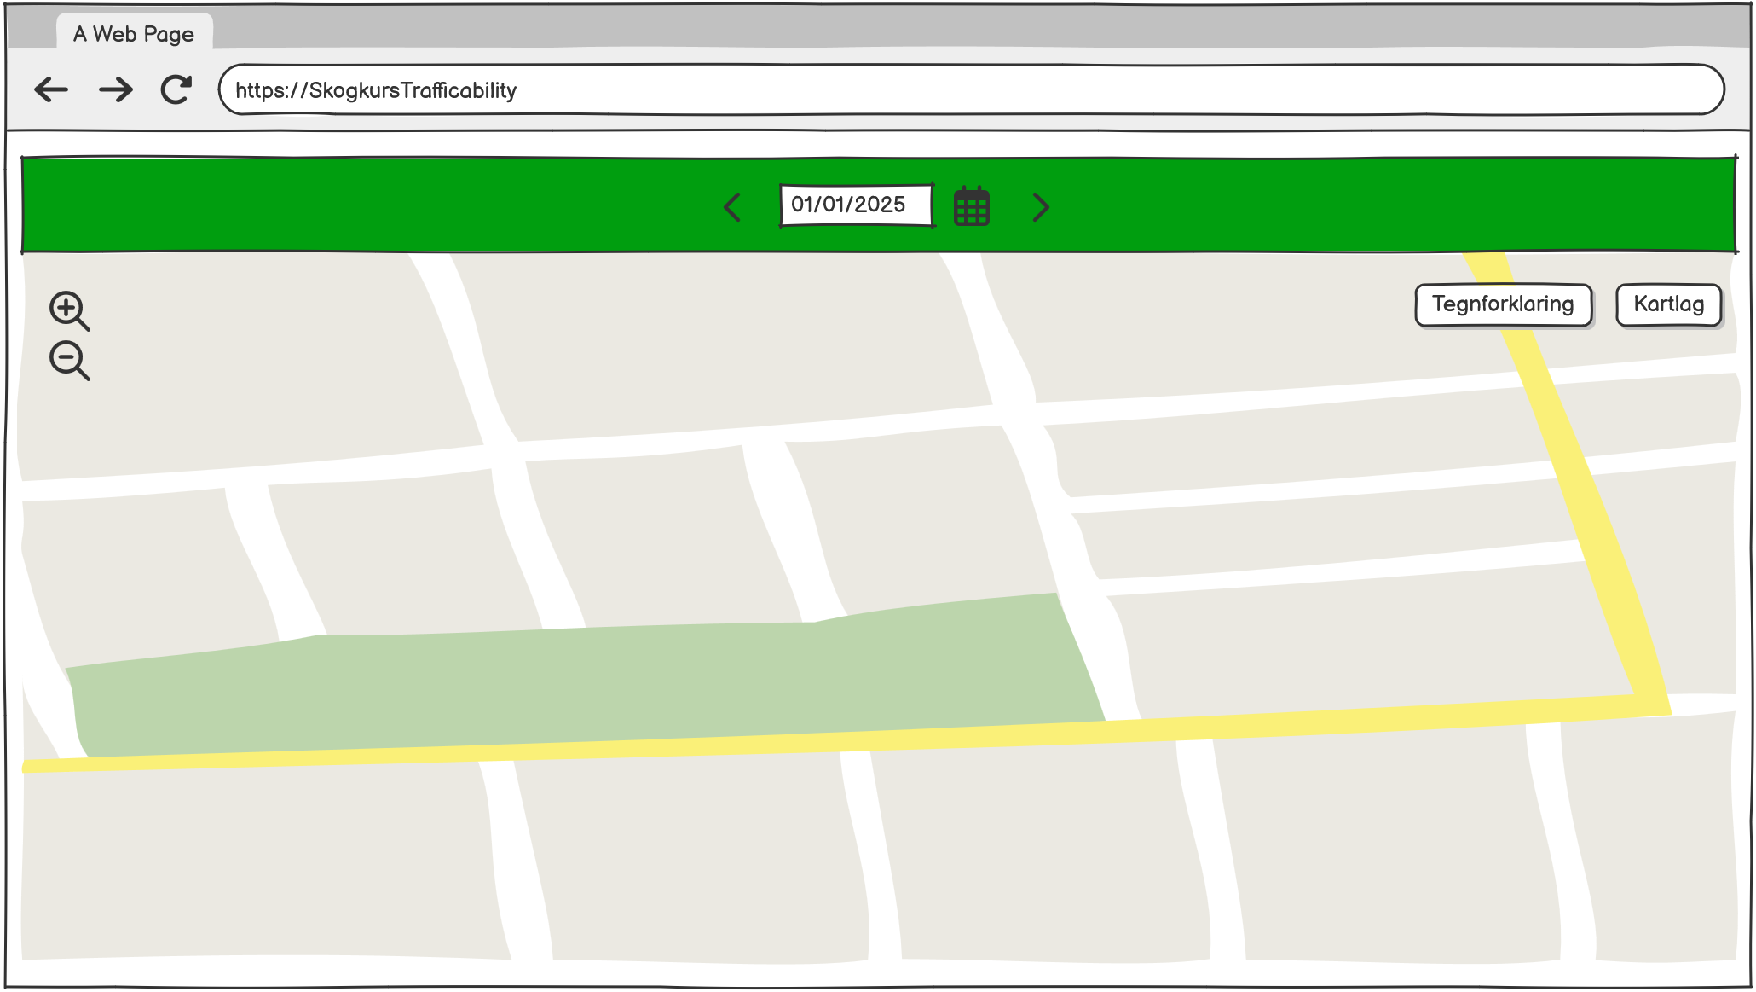
\includegraphics[width=0.6\linewidth]{figures/wireframe_website_sidebars_closed.pdf} 
    \caption{Wireframe of the website with no map layer enabled}
    \label{fig:wireframe_website_sidebars_closed}
\end{figure}

\begin{figure}[h]
    \centering
    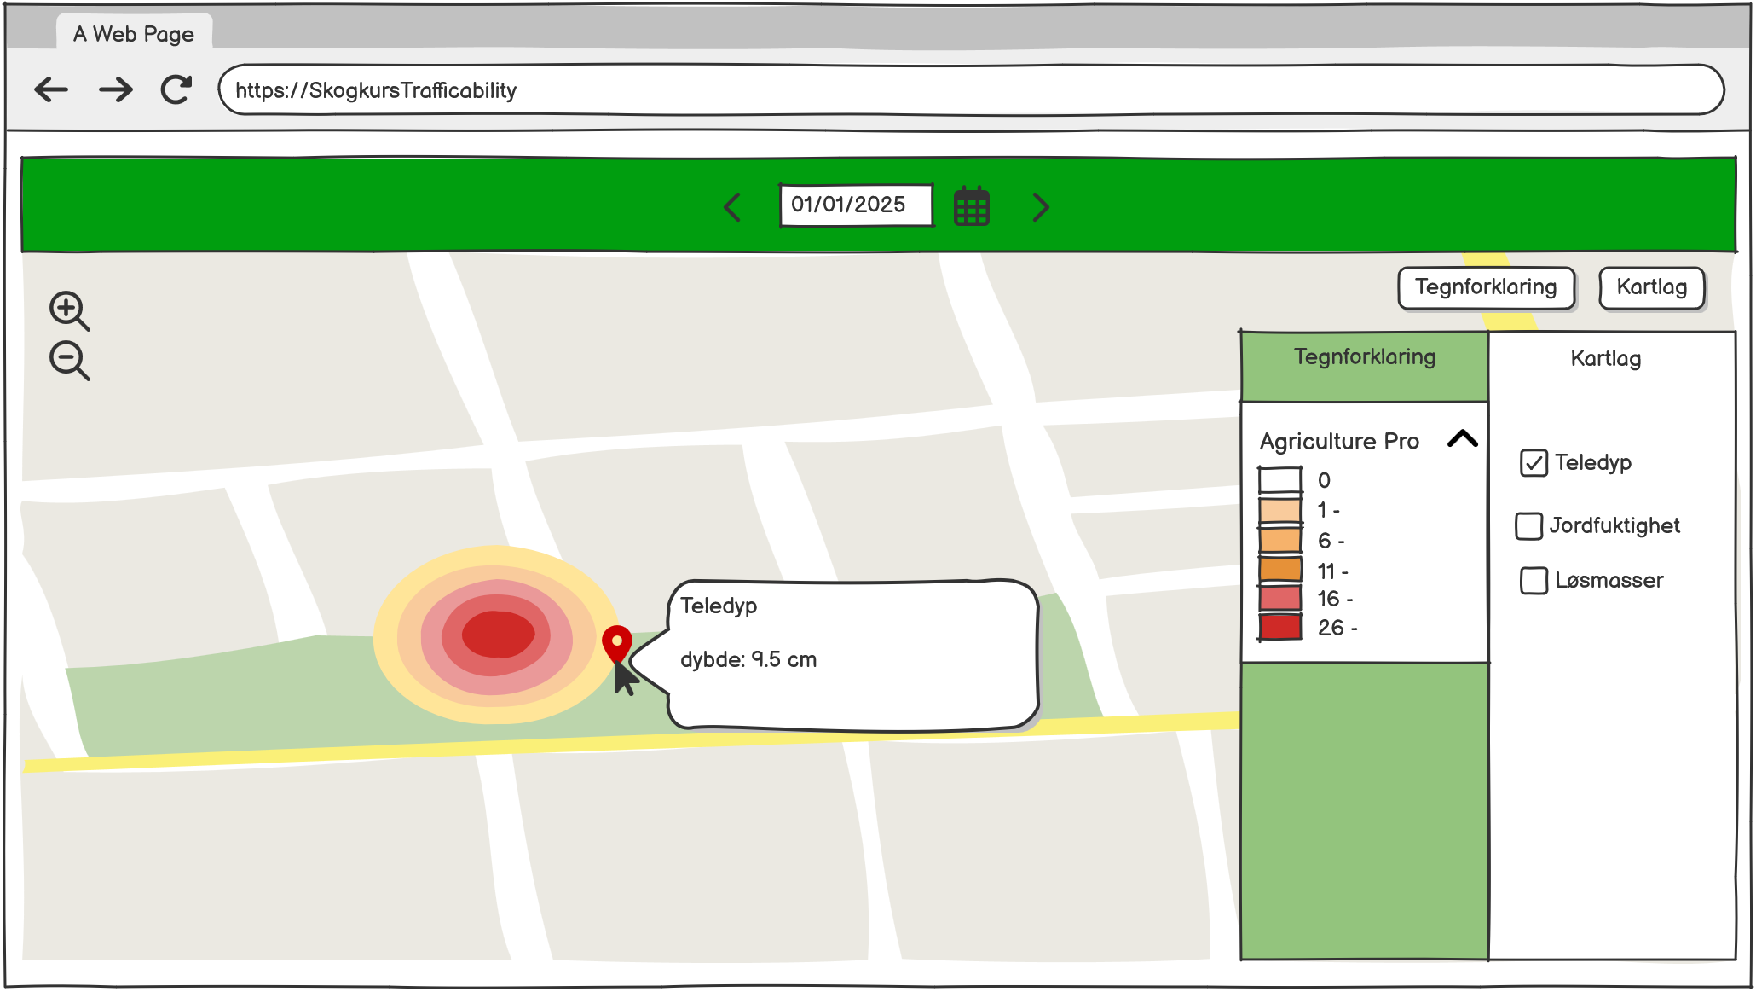
\includegraphics[width=0.6\linewidth]{figures/wireframe_website_sidebars_opened.pdf}
    \caption{Wireframe of the website with a map layer enable}
    \label{fig:wireframe_website_sidebars_opened}
\end{figure}

\subsection{UI Components}

\textcolor{orange}{NOE TEKST}
\begin{figure}[h]
    \centering
    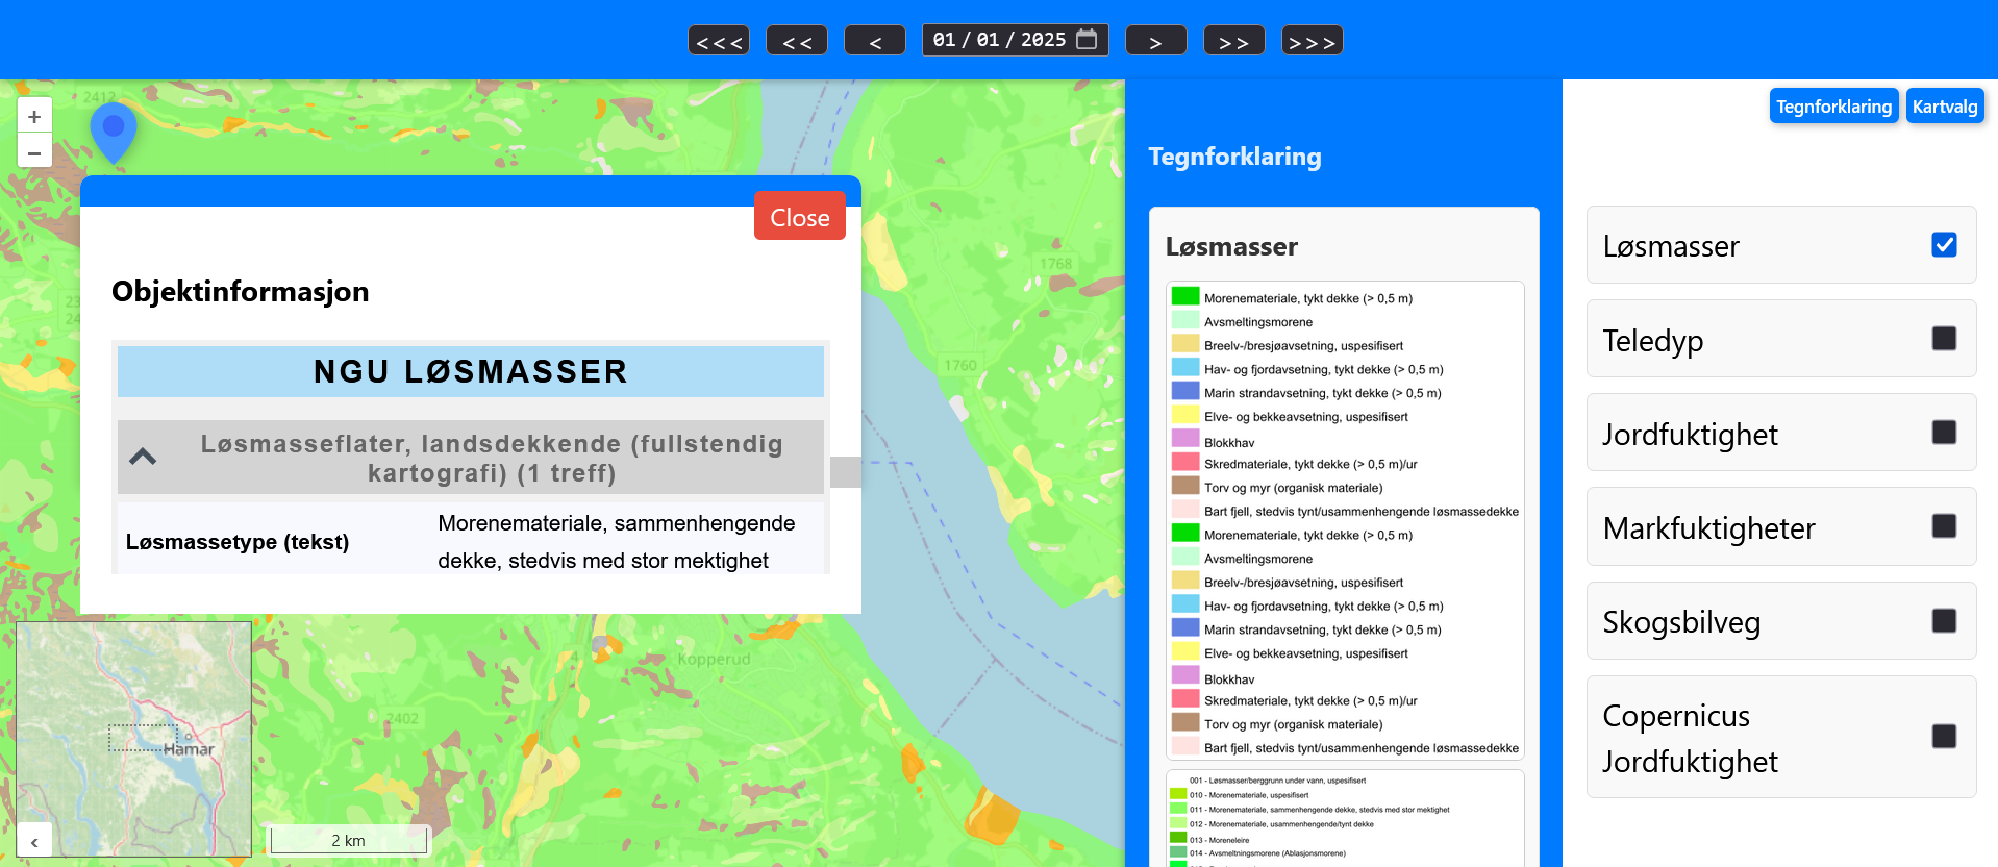
\includegraphics[width=1\linewidth]{figures/website_layout_v1.pdf}
    \caption{Early version of website}
    \label{fig:website_layout_v1}
\end{figure}

\subsection{Component State} % eller state management?

\textcolor{orange}{NOE TEKST}

\subsection{Map Layers}

\textcolor{orange}{NOE TEKST}

\subsection{Date Picker}

The date picker is used to change the current date of the data shown on the map. This lets the user see historical and forecast data. The component consists of an \acrshort{html} date input element and buttons to change the date by day, week or year. When the user changes the date, all enabled map layers will be updated with the new date and displayed on the map as long as they have data from that specific date.

\subsection{Trafficability Algorithm} 

% Processing Algorithm?
The roads are displayed in green, yellow, or red, indicating their trafficability. These classifications are based on calculations that incorporate both meteorological and geological data.

\textcolor{orange}{NOE TEKST}

\section{Server}

The backend server consists of TWO/THREE endpoints: a proxy for \Gls{wms} services, a query aggregator and the forestry road NOE. 
% Generelt om Server
The backend server is written in Go (REF/GLOSS) and designed as a REST API (REF/GLOSS). 

\begin{table}[h]
    \centering
    \begin{tabular}{|l|l|}
        \hline
        \textbf{Library} & \textbf{Description} \\
        \hline
        joho/godotenv & Loads environment variables from .env files. \\
        rs/zerolog & Zero Allocation Logger. \\
        tidwall/rtree & An R-tree implementation for spatial querying. \\
        twpayne/go-geom & Efficient geometry types for geospatial applications. \\
        twpayne/go-proj & Transformation between different coordinate systems. \\
        twpayne/go-shapefile & Native Go reader for ESRI Shapefiles \\
        \hline
    \end{tabular}
    \caption{Overview of used Go libraries}
    \label{tab:go_libraries}
\end{table}

\begin{comment}
\item[Implementation:] Here you should describe the more technical details of the solution. Which tools were used (programming languages, libraries, IDEs, APIs, frameworks, etc.). It is a good idea to give some code examples. If class diagrams, database models etc. were not presented in the technical design chapter, they can be included here.
    - Golang (libraries?)
    - Source of map layers/ legends (endpoint, etc.)
    - Proxy
    - Algorithm for trafficability of forest roads
\end{comment}

\subsection{Forestry Road Algorithm}

\textcolor{orange}{NOE TEKST}

\subsection{Proxy}\label{subsec:proxy}

As described in Section \ref{sec:systemarchitecture}, we wanted a clean architecture where all requests went through the backend server. 
\textcolor{orange}{NOE MER TEKST... HVORDAN IMPLEMENTERT, HVORDAN BRUKES DET}

% Hvordan proxien funker
% Hva er effekten av en slik proxy
    % slik at clienten snakker med website, og website snakker med verdenen gjennom backend serveren

\subsection{Optimization}

Early iterations of the forest road retrieval and processing algorithm were computationally expensive, resulting in long response times when querying the forest road layer.

\subsubsection{SeNorge}

The backend would initially query the SeNorge API once for every road, which would quickly overload the API server leading to long processing times. Additionally, the SeNorge API would not accept multiple coordinates within each grid-cell. SeNorge uses a grid system to divide Norway into \qty{1}{\kilo\meter\squared} cells, and calculate all their climate projections as an average within each cell \cite{senorge_watermap}. 

Lacking documentation of how the grid-cells were initially declared, in addition to a deprecated service for transforming coordinates to cell indexes, prompted further investigation into the SeNorge grid-cells. Findings showed that each grid-cell had borders that lined up with the UTM zone 33N projection system, where the latitude and longitude of each grid intersection were a multiple of \qty{1000}{}. In other words, each grid is centered on a UTM coordinate that is a multiple of $\qty{1000}{}\pm\qty{500}{}$.

The findings made it possible to cluster the forest roads into their closest SeNorge grid-cell, without explicitly knowing which grid-cell was closest. The coordinate of the cluster center could then be used to send a singular request to the SeNorge API, drastically increasing the amount of roads that could be processed at once. Listing \ref{lst:clusterforestroads} shows the implementation of the clustering, where the forest roads are clustered into a sharded map for fast concurrent read and writes.

% TODO: oppdater denne listingen med bedre kode
% (int(math.Round(coordinates[0])))????
\begin{figure}[H]
\lstinputlisting[
    caption={Clustering of forest roads},
    label=lst:clusterforestroads,
    language=Go
]{listings/clusterwfsresponsetoshardedmap.go}
\end{figure}

\subsubsection{Spatial querying}

Another large optimization was made related to how superficial deposit along the roads were queried. Initially, the middle of each road would be used to query the forestry road \Gls{wfs}, leading to a large amount of HTTP requests. These HTTP requests would then quickly overload the \Gls{wfs}, leading to extensive response times.

This was solved by downloading the superficial deposit data and reconstructing it into a map in-memory. The data was downloaded from GeoNorge\footnote{\url{https://kartkatalog.geonorge.no/}} and is availbable under the NLOD license\footnote{\url{https://data.norge.no/nlod/no/2.0}}. 

\textcolor{orange}{Noe mer tekst om hvordan vi har implementert det, og hvorfor vi valgte denne implementasjonen.}

\begin{figure}[h]
\lstinputlisting[
    caption={Building of spatial index},
    label=lst:spatialindex,
    language=Go
]{listings/readshapefileandbuildindex.go}
\end{figure}

% Rtree ble brukt for å ha effektiv querying av spatial data. Skulle egentlig bruke querying av WMS, men fant fort ut at det var urealistisk med så mange requests (NEVNE SENORGE AT DE VAR 1KM, mens vi ville a per 50m eller mindre). I tilegg var dataen om løsmasser tilgjengelig under NLOD, så en in-memory løsning ville funke. R-tree ble derfor valgt ettersom det er en effektiv datastruktur for querying of spatial data. Implementasjonen bygger et r-tree fra SHAPE filer.

\subsubsection{Goroutines}

\textcolor{orange}{Antall veier som må bli prosessert avhenger av hvor zoomet inn man er på kartet, og vil noen ganger inneholde flere tusen del-veier på en gang. Å prosessere hver av disse sekvensielt ville tatt for lang tid, så pararell prosessering måtte bli tatt i bruk. Som nevnt over i kapittelet techologies/go har go en sterk fordel med goroutines, som er lightweight multithreading. Goroutines blir brukt flere steder, som querying av løsmasser og som i code listing 5.1 for clustering av veier. }
% Det er allikevel viktig å passe på at alle goroutines har en klar måte å exite på, eller en måte å bli signalisert til å stoppe.

% Hva er problemet?
% Hva er goroutines og hvorfor er det bra for oss?
% Hvordan vi bruker det

\begin{comment}
UTFORDRINGER OM IMPLEMENTASJON HER:
    - Kilder
        - Senorge dårlig dokumentasjon til API
            - Bruker annen endpoint istedenfor
    - Finne gode og nøyaktige data
    - Gjøre om data til WMS/noe vi kan vise
    - Gjøre om WMS/kartdata til rød, grønn eller gule veier
    - Konvertering av koordinater, f.eks. fra epsg:3857 til epsg:25833
    - Klassifisering av skogsbilveger
        - Hente teledyp data for flere veger (WMS vs. REST API)
        - Teletyp var vanskeligere enn forventet siden API-en brukte et dårlig dokumentert grid-system.
\end{comment}
